\subsection{FUNCTORIAL PROPERTIES OF THE EXTERIOR ALGEBRA}

PROPOSITION 2. Let A be a commutative ring, M and N two A-modules and u: M → N an A-linear mapping. There exists one and only one A-algebra homomorphism

\[
u ^ {\prime \prime}: \bigwedge (\mathbf {M}) \rightarrow \bigwedge (\mathbf {N})
\]

such that the diagram

\pandocbounded{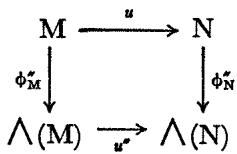
\includegraphics[keepaspectratio]{images/part003_b216bf24.jpg}}

is commutative. Moreover, \(u''\) is a graded algebra homomorphism.

The existence and uniqueness of \(u''\) follow from no. 1, Proposition 1 applied to the algebra \(\bigwedge(\mathbf{N})\) and \(f = \phi_{\mathbf{N}}'' \circ u: \mathbf{M} \to \bigwedge(\mathbf{N})\) ; for \(f(\mathbf{M}) \subset \mathbf{N}\) and hence \(f\) satisfies condition (1) by definition of \(\mathfrak{J}_{\mathbf{N}}''\) : as \(f(\mathbf{M}) \subset \bigwedge^{1}(\mathbf{N}) = \mathbf{N}\) , the fact that \(u''\) is a graded algebra homomorphism follows from Remark 1 of no. 1.

The homomorphism \(u''\) of Proposition 2 will henceforth be denoted by \(\bigwedge(u)\) . If P is an A-module and \(v: \mathbf{N} \to \mathbf{P}\) is an A-linear mapping, then

\[
\bigwedge (v \circ u) = \bigwedge (v) \circ \bigwedge (u)\tag{3}
\]

for \(\bigwedge(v) \circ \bigwedge(u)\) is an algebra homomorphism which renders commutative the diagram

\pandocbounded{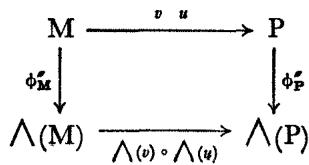
\includegraphics[keepaspectratio]{images/part003_3a522f8d.jpg}}

Since \(\bigwedge (\mathbf{M})\) contains \(\mathbf{M} = \bigwedge^{1}(\mathbf{M}),\bigwedge (u)\) is sometimes called the canonical extension of \(u\) to \(\bigwedge (\mathbf{M})\) . The restriction \(\bigwedge^n (u):\bigwedge^n (\mathbf{M})\to \bigwedge^n (\mathbf{N})\) is such that

\[
\bigwedge^ {n} (u) (x _ {1} \land x _ {2} \land \dots \land x _ {n}) = u (x _ {1}) \land u (x _ {2}) \land \dots \land u (x _ {n})\tag{4}
\]

with the \(x_{i}\in\mathbf{M}\) , since \(\bigwedge(u)\) is an algebra homomorphism and \(\bigwedge^{1}(u)=u\) ; the restriction \(\bigwedge^{0}(u)\) to A is the identity mapping. Note that \(\bigwedge^{n}(u)\) is obtained from \(\mathsf{T}^{n}(u):\mathsf{T}^{n}(\mathbf{M})\to\mathsf{T}^{n}(\mathbf{N})\) by passing to the quotients.

PROPOSITION 3. If \(u: \mathbf{M} \to \mathbf{N}\) is a surjective A-linear mapping, the homomorphism \(\bigwedge(u): \bigwedge(\mathbf{M}) \to \bigwedge(\mathbf{N})\) is surjective and its kernel is the two-sided ideal of \(\bigwedge(\mathbf{M})\) generated by the kernel \(\mathbf{P} \subset \mathbf{M} \subset \bigwedge(\mathbf{M})\) of \(u\) .

The proof is derived from that of §6, no. 2, Proposition 4, replacing S by \(\bigwedge\) and \(\mathfrak{J}'\) by \(\mathfrak{J}''\) .

If \(u: \mathbf{M} \to \mathbf{N}\) is an injective linear mapping, it is not always true that \(\bigwedge(\mathbf{u})\) is an injective mapping (§ 6, Exercise 3) (see however below no. 9, Corollary to Proposition 12). However this is so when \(u\) is an injection such that \(u(\mathbf{M})\) is a direct factor of \(\mathbf{N}\) and then the image of \(\bigwedge(u)\) (isomorphic to \(\bigwedge(\mathbf{M})\) ) is a direct factor of \(\bigwedge(\mathbf{N})\) ; the proof is the same as that for the analogous assertions for \(\mathbf{T}(u)\) (§ 5, no. 2) replacing \(\mathbf{T}\) by \(\bigwedge\) .

PROPOSITION 4. Let N and P be two submodules of an A-module M such that their sum N + P is a direct factor in M and their intersection N ∩ P is a direct factor in N and in P. Then the homomorphisms \(\bigwedge(\mathrm{N}) \to \bigwedge(\mathrm{M})\) , \(\bigwedge(\mathrm{P}) \to \bigwedge(\mathrm{M})\) and \(\bigwedge(\mathrm{N} \cap \mathrm{P}) \to \bigwedge(\mathrm{M})\) , canonical extensions of the canonical injections, are injective; if \(\bigwedge(\mathrm{N})\) , \(\bigwedge(\mathrm{P})\) and \(\bigwedge(\mathrm{N} \cap \mathrm{P})\) are identified with subalgebras of \(\bigwedge(\mathrm{M})\) by means of these homomorphisms, then

\[
\bigwedge (\mathbf {N} \cap \mathbf {P}) = \bigwedge (\mathbf {N}) \cap \bigwedge (\mathbf {P}).\tag{5}
\]

The proof is derived from that of § 5, no. 2, Proposition 4 replacing T by \(\bigwedge\) throughout. The hypotheses of Proposition 4 are always satisfied by arbitrary submodules N, P of M when A is a field.

COROLLARY. Let K be a commutative field and M a vector space over K. For every element \(z \in \bigwedge(\mathbf{M})\) , there exists a smallest vector subspace N of M such that \(z \in \bigwedge(\mathbf{N})\) and N is finite-dimensional.

The proof is deduced from that of § 5, no. 2, Corollary to Proposition 4 replacing T by \(\bigwedge\) throughout.

N is called the vector subspace of M associated with the element z of \(\bigwedge(\mathbf{M})\) .
% semantic-fragments: legacy-input-seam
\relax{}
